% **** Szablon pracy magisterskiej, licencjackiej lub inżynierskiej ****

\documentclass[polish,12pt,twoside,a4paper]{report}

% *************** Definicje stylu dokumentu ***************

% *********************************************************************************
% W pliku tym zdefiniowany jest wygl¹d dokumentu.
% Zmiany tutaj nie s¹ konieczne o ile nie zamierzasz zmieniaæ wygl¹du dokumentu.
% *********************************************************************************

% *************** Za³adowanie pakietów ***************
\usepackage[a4paper,twoside,left=2.0cm,right=1.5cm,top=1.5cm,bottom=1.5cm]{geometry}
\usepackage[T1]{fontenc}
%\usepackage[cp1250]{inputenc}
\usepackage[utf8]{inputenc}
\usepackage[polish]{babel}
\usepackage{amsmath}
\usepackage{amsfonts}
\usepackage{graphicx}
\usepackage{graphics}
\usepackage{times}
\usepackage{indentfirst}%wciecia a nowych akapitach

\selectlanguage{polish}

%szerokoœœ wciêæ
\setlength{\parindent}{1.25cm}

%numeracja stron
\usepackage{fancyhdr}
\pagestyle{fancy}
\fancyhf{} % usun biezace ustawienia pagin
\fancyhead[LE,RO]{ }
\fancyhead[LO]{ }
\fancyhead[RE]{ }
\fancyfoot[LE,RO]{\small\thepage}
\fancyfoot[LO]{ }
\fancyfoot[RE]{ }
\renewcommand{\headrulewidth}{0.0pt}
\renewcommand{\footrulewidth}{0.0pt}
\addtolength{\headheight}{0.0pt} % pionowy odstep na kreske
\fancypagestyle{plain}{%
\fancyhead{} % usun p. górne na stronach pozbawionych
% numeracji (plain)
\renewcommand{\headrulewidth}{0.0pt} % pozioma kreska
}

% *************** Definicje niektórych kolorów ***************
\usepackage{color}

\definecolor{greenyellow}   {cmyk}{0.15, 0   , 0.69, 0   }
\definecolor{yellow}        {cmyk}{0   , 0   , 1   , 0   }
\definecolor{goldenrod}     {cmyk}{0   , 0.10, 0.84, 0   }
\definecolor{dandelion}     {cmyk}{0   , 0.29, 0.84, 0   }
\definecolor{apricot}       {cmyk}{0   , 0.32, 0.52, 0   }
\definecolor{peach}         {cmyk}{0   , 0.50, 0.70, 0   }
\definecolor{melon}         {cmyk}{0   , 0.46, 0.50, 0   }
\definecolor{yelloworange}  {cmyk}{0   , 0.42, 1   , 0   }
\definecolor{orange}        {cmyk}{0   , 0.61, 0.87, 0   }
\definecolor{burntorange}   {cmyk}{0   , 0.51, 1   , 0   }
\definecolor{bittersweet}   {cmyk}{0   , 0.75, 1   , 0.24}
\definecolor{redorange}     {cmyk}{0   , 0.77, 0.87, 0   }
\definecolor{mahogany}      {cmyk}{0   , 0.85, 0.87, 0.35}
\definecolor{maroon}        {cmyk}{0   , 0.87, 0.68, 0.32}
\definecolor{brickred}      {cmyk}{0   , 0.89, 0.94, 0.28}
\definecolor{red}           {cmyk}{0   , 1   , 1   , 0   }
\definecolor{orangered}     {cmyk}{0   , 1   , 0.50, 0   }
\definecolor{rubinered}     {cmyk}{0   , 1   , 0.13, 0   }
\definecolor{wildstrawberry}{cmyk}{0   , 0.96, 0.39, 0   }
\definecolor{salmon}        {cmyk}{0   , 0.53, 0.38, 0   }
\definecolor{carnationpink} {cmyk}{0   , 0.63, 0   , 0   }
\definecolor{magenta}       {cmyk}{0   , 1   , 0   , 0   }
\definecolor{violetred}     {cmyk}{0   , 0.81, 0   , 0   }
\definecolor{rhodamine}     {cmyk}{0   , 0.82, 0   , 0   }
\definecolor{mulberry}      {cmyk}{0.34, 0.90, 0   , 0.02}
\definecolor{redviolet}     {cmyk}{0.07, 0.90, 0   , 0.34}
\definecolor{fuchsia}       {cmyk}{0.47, 0.91, 0   , 0.08}
\definecolor{lavender}      {cmyk}{0   , 0.48, 0   , 0   }
\definecolor{thistle}       {cmyk}{0.12, 0.59, 0   , 0   }
\definecolor{orchid}        {cmyk}{0.32, 0.64, 0   , 0   }
\definecolor{darkorchid}    {cmyk}{0.40, 0.80, 0.20, 0   }
\definecolor{purple}        {cmyk}{0.45, 0.86, 0   , 0   }
\definecolor{plum}          {cmyk}{0.50, 1   , 0   , 0   }
\definecolor{violet}        {cmyk}{0.79, 0.88, 0   , 0   }
\definecolor{royalpurple}   {cmyk}{0.75, 0.90, 0   , 0   }
\definecolor{blueviolet}    {cmyk}{0.86, 0.91, 0   , 0.04}
\definecolor{periwinkle}    {cmyk}{0.57, 0.55, 0   , 0   }
\definecolor{cadetblue}     {cmyk}{0.62, 0.57, 0.23, 0   }
\definecolor{cornflowerblue}{cmyk}{0.65, 0.13, 0   , 0   }
\definecolor{midnightblue}  {cmyk}{0.98, 0.13, 0   , 0.43}
\definecolor{navyblue}      {cmyk}{0.94, 0.54, 0   , 0   }
\definecolor{royalblue}     {cmyk}{1   , 0.50, 0   , 0   }
\definecolor{blue}          {cmyk}{1   , 1   , 0   , 0   }
\definecolor{cerulean}      {cmyk}{0.94, 0.11, 0   , 0   }
\definecolor{cyan}          {cmyk}{1   , 0   , 0   , 0   }
\definecolor{processblue}   {cmyk}{0.96, 0   , 0   , 0   }
\definecolor{skyblue}       {cmyk}{0.62, 0   , 0.12, 0   }
\definecolor{turquoise}     {cmyk}{0.85, 0   , 0.20, 0   }
\definecolor{tealblue}      {cmyk}{0.86, 0   , 0.34, 0.02}
\definecolor{aquamarine}    {cmyk}{0.82, 0   , 0.30, 0   }
\definecolor{bluegreen}     {cmyk}{0.85, 0   , 0.33, 0   }
\definecolor{emerald}       {cmyk}{1   , 0   , 0.50, 0   }
\definecolor{junglegreen}   {cmyk}{0.99, 0   , 0.52, 0   }
\definecolor{seagreen}      {cmyk}{0.69, 0   , 0.50, 0   }
\definecolor{green}         {cmyk}{1   , 0   , 1   , 0   }
\definecolor{forestgreen}   {cmyk}{0.91, 0   , 0.88, 0.12}
\definecolor{pinegreen}     {cmyk}{0.92, 0   , 0.59, 0.25}
\definecolor{limegreen}     {cmyk}{0.50, 0   , 1   , 0   }
\definecolor{yellowgreen}   {cmyk}{0.44, 0   , 0.74, 0   }
\definecolor{springgreen}   {cmyk}{0.26, 0   , 0.76, 0   }
\definecolor{olivegreen}    {cmyk}{0.64, 0   , 0.95, 0.40}
\definecolor{rawsienna}     {cmyk}{0   , 0.72, 1   , 0.45}
\definecolor{sepia}         {cmyk}{0   , 0.83, 1   , 0.70}
\definecolor{brown}         {cmyk}{0   , 0.81, 1   , 0.60}
\definecolor{tan}           {cmyk}{0.14, 0.42, 0.56, 0   }
\definecolor{gray}          {cmyk}{0   , 0   , 0   , 0.50}
\definecolor{black}         {cmyk}{0   , 0   , 0   , 1   }
\definecolor{white}         {cmyk}{0   , 0   , 0   , 0   } 

% *************** Koniec definicji stylu dokumentu ***************


%definicja przydatnych poleceń
\newcommand{\wydzial}{KOLEGIUM INFORMATYKI STOSOWANEJ}
\newcommand{\kierunek}{Kierunek: INFORMATYKA}
\newcommand{\specjalnosc}{Specjalność: Programowanie}
\newcommand{\autor}{Adrian Zachwiej}
\newcommand{\album}{Nr albumu studenta w56233}
\newcommand{\temat}{Program Kuchenka Mikrofalowa}
\newcommand{\promotor}{mgr inż. Ewa Żesławska}
\newcommand{\typpracy}{Projekt}
\newcommand{\miasto}{Rzeszów}
\newcommand{\rok}{2024}

\begin{document}

% *************** Włączenie definicji pierwszych stron ***************
% *************** Strony tytułowe ***************

% ************************************************************
% W tym miejscu znajduje sie definicja wyglądu pierwszych stron:
% strony tytułowej, strony z oświadczeniem o treści pracy
% i strony ze spisem treści
% ************************************************************
% *************** Strona tytułowa ***************
%umieszczenie logo i nazwy uczelni
\noindent
\parbox{65mm}{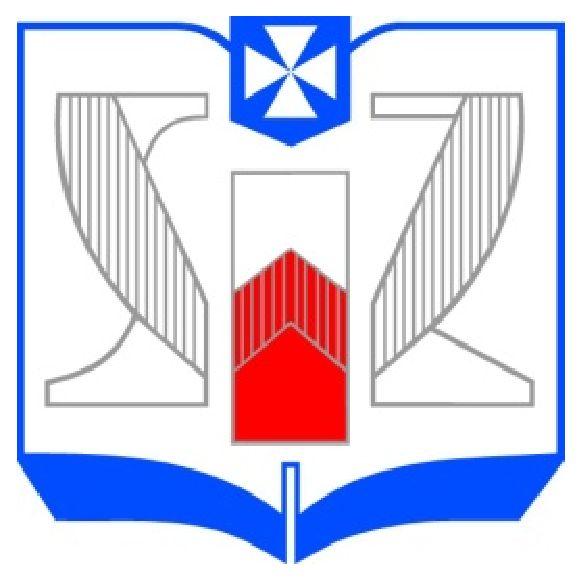
\includegraphics[width=13.0cm, height=3.0cm]{logoWSIiZ}}

\vspace{10mm}
\begin{center}
{\Large{}\textbf{\wydzial}}
\end{center}
\vspace{10mm}
\noindent
\hspace{30mm}{\Large{}\textbf{\kierunek}}\\

\noindent
\hspace{30mm}{\Large{}\textbf{\specjalnosc}}
\vspace{30mm}
\begin{center}
	{\large{}\autor}\\
	{\large{}\album}\\
	\vspace{15pt}
	{\huge{}\textbf{\textit{\temat}}}\\
	\vspace{20pt}
	{\normalsize{}Promotor: \promotor}\\
	\vspace{100pt}
	{\LARGE{}\textbf{\typpracy}}\\
	\vspace{190pt}
	{\large{}\textbf{\miasto {} \rok}}
\end{center}

% pusta zawartość stopki - brak numeru strony
\thispagestyle{empty}

% *************** Strona z oświadczeniem o treści pracy ***************
\newpage
\text{}

\thispagestyle{empty}
\newpage


% *************** Spis treści ***************
\tableofcontents
% pusta zawartość stopki - brak numeru strony
\thispagestyle{empty}
\newpage

% *************** Koniec pliku front.tex ***************



% *************** Część główna pracy ***************
\chapter*{Wstęp}

\section*{Opis Projektu}
Dokumentacja dotyczy projektu futurystycznej kuchenki mikrofalowej, która posiada bazę danych typów jedzenia, prowadzi historię podgrzewań, przeprowadza samodiagnostykę, wymaga czyczeczenia po pięciu użyciach.

\section*{Cele Projektu}
Głównym celem projektu jest:
\begin{itemize}
    \item Stworzenie konsoli obsługi kuchenki mikrofalowej.
    \item Zapewnienie dostępu do danych przechowywanych na temat typów jedzenia.
    \item Zwiększenie efektywności obsługi danych i mikrofalówki.
\end{itemize}

\section*{Założenia Projektowe}
Podstawowe założenia projektu obejmują:
\begin{itemize}
    \item Możliwość dodawania, wyświetlania, aktualizacji i usuwania danych jedzenia.
    \item Możliwość przeprowadzenia diagnostyki i naprawy w razie potrzeby kuchenki mikrofalowej.
    \item Prowadzenie historii podgrzewań.
\end{itemize}

\addcontentsline{toc}{chapter}{Wstęp}
\newpage
% ********** Rozdział 0 **********
\chapter{Wymagania projektu}
\section{Wymagania Funkcjonalne}

\begin{enumerate}
    \item \textbf{Rozpoczęcie podgrzewania:} \\
     Użytkownik może wybrać produkt z listy dostępnych produktów, wprowadzić czas gotowania w sekundach.
    
    \item \textbf{Informacja z podgrzewania:} \\
    Użytkownik może przerwać podgrzewanie, po zakończeniu gotowania użytkownik otrzymuje informację o stanie gotowania (np. czy jedzenie jest spalone, niedogotowane lub gotowe).
    
    \item \textbf{Zarządzanie produktami:} \\
    Użytkownik może dodawać nowe produkty do listy dostępnych produktów wraz z czasem gotowania, usuwać istniejące produkty, edytować istniejące produkty.
    
    \item \textbf{Historia użycia:} \\
    Mikrofalówka rejestruje historię każdego użycia, wraz z informacjami o produkcie, czasie gotowania i wyniku (np. czy jedzenie było gotowe, niedogotowane lub spalone), użytkownik może przeglądać historię użycia.
    
    \item \textbf{Czyszczenie mikrofalówki:} \\
    Po każdych pięciu użyciach mikrofalówka wymaga czyszczenia, użytkownik może zresetować licznik użycia po wykonaniu czyszczenia.
    
    \item \textbf{Interfejs użytkownika:} \\
    Użytkownik powinien mieć prosty interfejs do nawigacji po funkcjach mikrofalówki. Po zakończeniu operacji użytkownik powinien mieć możliwość powrotu do głównego menu.
\end{enumerate}

\newpage
\section{Wymagania Niefunkcjonalne}

\begin{enumerate}
    \item \textbf{Wydajność:} \\
    Mikrofalówka powinna być responsywna i szybka w działaniu, zapewniając użytkownikowi płynne doświadczenie użytkowania.
    
    \item \textbf{Diagnostyka:} \\
    Mikrofalówka powinna być poddana testom jednostkowym, aby zapewnić wysoką jakość i niezawodność działania.
    
    \item \textbf{Skalowalność:} \\
    Projekt mikrofalówki powinien być zaprojektowany w taki sposób, aby łatwo można było dodawać nowe funkcje i rozszerzać jego możliwości w przyszłości.
    
    \item \textbf{Skalowalność:} \\
    System powinien być łatwo skalowalny, umożliwiając dostosowanie się do wzrostu liczby klientów i zwiększenia obciążenia systemu. Architektura systemu powinna być elastyczna i umożliwiać dodawanie nowych zasobów w miarę potrzeb.
    
    \item \textbf{Dostępność:} \\
    Aplikacja mikrofalówki powinna być dostępna dla osób z różnymi poziomami umiejętności.
    
\end{enumerate}



% ********** Koniec rozdziału **********

\newpage
% ********** Rozdział 1 **********
\chapter{Opis struktury projektu}
\section{Diagram Klas}
\begin{figure}[h]
    \centering
    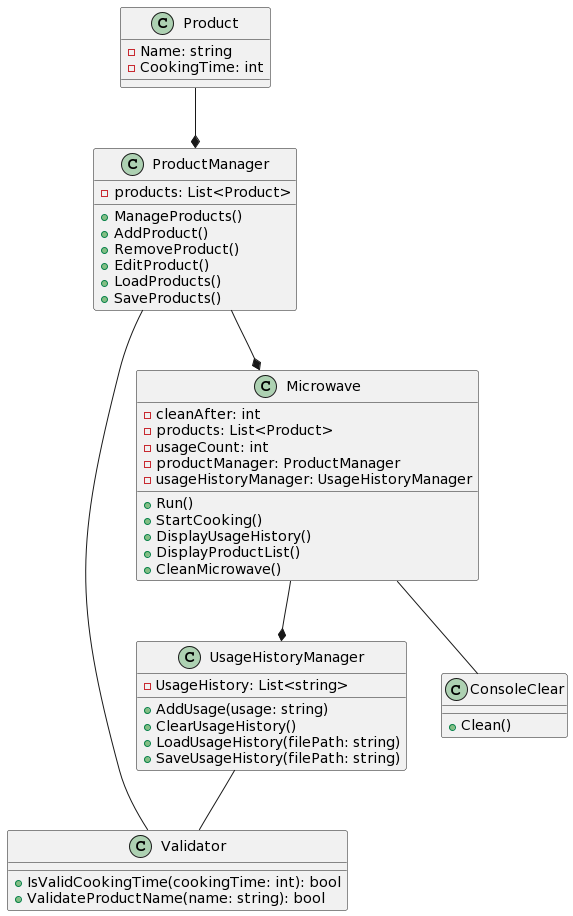
\includegraphics[width=0.7\textwidth]{Diagram.png}
      \caption{Diagram Klas - Opis projektu}
    \label{fig:example}
\end{figure}

\newpage

\section{Opis Diagramu Klas}

Diagram klas przedstawia system kuchenki mikrofalowej. Składa się on z klas oraz relacji między nimi.

\subsection{Klasy}

\begin{itemize}
  \item \textbf{Product}: Klasa reprezentująca produkt, który może być podgrzewany w mikrofalówce. Posiada właściwości Name (nazwa produktu) i CookingTime (czas podgrzewania).
  \item \textbf{ProductManager}: Zarządza produktami dostępnymi w mikrofalówce. Posiada listę produktów oraz metody do dodawania, usuwania, edycji, ładowania i zapisywania produktów. Wykorzystuje walidację produktów za pomocą klasy Validator.
  \item \textbf{Validator}: Klasa narzędziowa do walidacji danych, takich jak poprawność czasu podgrzewania i nazwy produktu.
  \item \textbf{Microwave}: Główna klasa reprezentująca mikrofalówkę. Zarządza procesem gotowania, wyświetlaniem historii użycia, zarządzaniem produktami, czyszczeniem mikrofalówki i diagnostyką.  Wykorzystuje obiekty klas ProductManager, UsageHistoryManager i ConsoleClear.
  \item \textbf{UsageHistoryManager}: Zarządza historią użycia mikrofalówki. Przechowuje listę zdarzeń użytkowania, z możliwością dodawania, czytania, czyszczenia, ładowania i zapisywania historii.
  \item \textbf{ConsoleClear}: Klasa narzędziowa do czyszczenia konsoli po zakończeniu operacji.
\end{itemize}


\subsection{Relacje}

\begin{itemize}
  \item Klasa Product jest wykorzystywana przez ProductManager, który zarządza nimi.
  \item ProductManager korzysta z klasy Validator do walidacji danych produktu.
  \item Microwave wykorzystuje ProductManager do zarządzania produktami, korzysta z UsageHistoryManager do zarządzania historią użytkowania, ConsoleClear do czyszczenia konsoli po zakończeniu operacji.
\end{itemize}
% ********** Koniec rozdziału **********

\newpage
% ********** Rozdział 2 **********
\chapter{Opis techniczny projektu}
\section{Wykorzystywane technologie}

Projekt został zaimplementowany w języku C\# z wykorzystaniem platformy .NET. Do zarządzania bazą danych używa plików tekstowych. Projekt wykorzystuje podejście programowania obiektowego.

\subsection{Narzędzia}
Do implementacji projektu użyto następujących narzędzi:
\begin{itemize}
    \item Microsoft Visual Studio - środowisko programistyczne do tworzenia aplikacji w języku C\#.
    \item LaTeX - do tworzenia dokumentacji w formacie PDF zgodnej z wymaganiami.
\end{itemize}
\subsection{Minimalne wymagania sprzętowe}
Minimalne wymagania sprzętowe dla uruchomienia projektu są następujące:
\begin{itemize}
    \item Procesor: Procesor zgodny z architekturą x86 lub x64 o częstotliwości 1 GHz lub więcej.
    \item Minimum 512 MB RAM.
    \item Minimum 100 MB wolnego miejsca na dysku twardym.
    \item  Windows 7 lub nowszy, lub dowolny system obsługujący środowisko uruchomieniowe .NET Framework 4.7.2 lub nowsze.
\end{itemize}
\subsection{Zarządzanie danymi oraz baza danych}

Do zarządzania danymi w projekcie wykorzystano klase ProductManager, zaimplementowano metody obsługujące operacje CRUD (Create, Read, Update, Delete) na tekstowej bazie danych. Klasa Validator sprawdza poprawność wprowadzonych danych.

% ********** Koniec rozdziału **********

\newpage
% ********** Rozdział 3 **********
\chapter{Harmonogram realizacji projektu}

Harmonogram realizacji projektu "System zarządzania kontem klienta w firmie telekomunikacyjnej" został stworzony w celu zaplanowania i kontrolowania procesu implementacji systemu oraz jego poszczególnych funkcjonalności. Harmonogram obejmuje szereg etapów, w których uwzględniono zadania związane z analizą wymagań, projektowaniem, implementacją, testowaniem i wdrożeniem systemu.

\section{Diagram Gantta}
\begin{figure}[h]
    \centering
    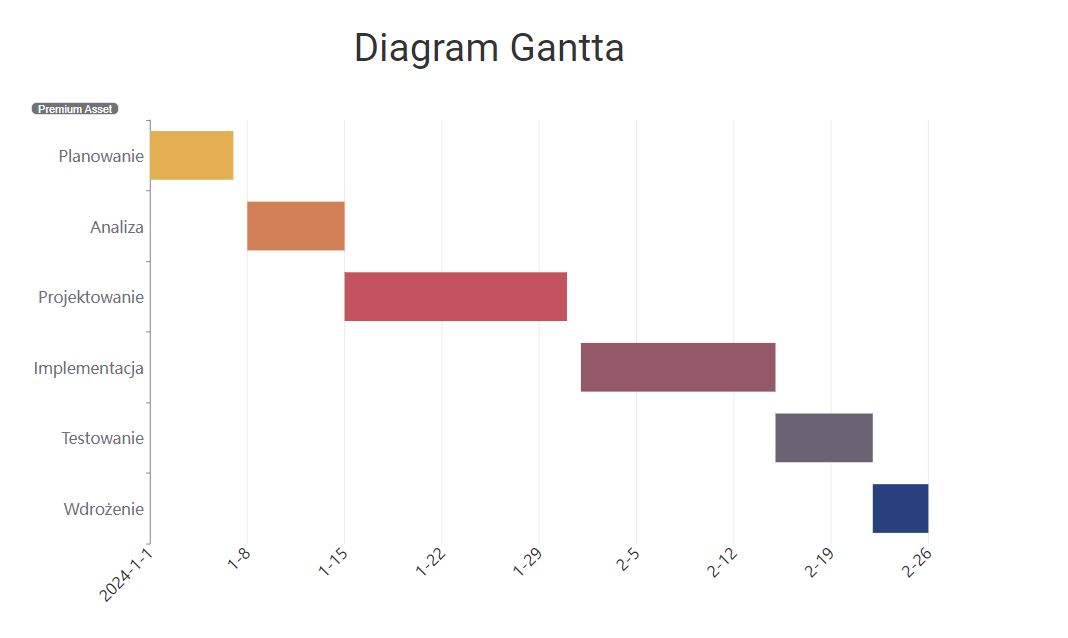
\includegraphics[width=\textwidth]{Gantt.png}
      \caption{Diagram Gantta - Opis realizacji projektu}
    \label{fig:example}
\end{figure}

\newpage

\subsection{Projektowanie (1/01/2024 - 7/01/2024)}
\begin{itemize}
    \item Zdefiniowanie funkcjonalnych i niefunkcjonalnych wymagań systemu.

\end{itemize}

\subsection{Analiza (8/01/2024 - 15/01/2024)}
\begin{itemize}
    \item Określenie oczekiwanych funkcji i interfejsu użytkownika
\end{itemize}

\subsection{Projektowanie (15/01/2024 - 31/01/2024)}
\begin{itemize}
    \item Opracowanie architektury systemu i struktury bazy danych.
    \item Utworzenie diagramów klas, schematów bazodanowych oraz interfejsów użytkownika.
    \item Sporządzenie dokumentacji projektowej i specyfikacji technicznej.
\end{itemize}

\subsection{implementacja (1/02/2024 - 15/02/2024)}
\begin{itemize}
    \item Pisanie kodu.
    \item Wprowadzanie poprawek do kodu i implementowanie kolejnych funkcjonalności.
\end{itemize}

\subsection{Testowanie (15/02/2024 - 22/02/2024)}
\begin{itemize}
    \item Przeprowadzenie testów funkcjonalnych i niefunkcjonalnych.
    \item Debugowanie i poprawa ewentualnych błędów.
\end{itemize}

\subsection{Wdrożenie (22/02/2024 - 26/02/2024)}
\begin{itemize}
    \item Prowadzenie testów integracyjnych i ostateczne dostosowanie systemu.
\end{itemize}

Harmonogram realizacji projektu jest elastyczny i może ulec zmianie w razie konieczności dostosowania do zmieniających się warunków lub potrzeb projektowych.


% ********** Koniec rozdziału **********

\newpage
\chapter{Repozytorium i system kontroli wersji}

GitHub to platforma do udostępniania projektów programistów a nawet projektów całych zepsołów programistków. Oferuje wiele narzedzi umożliwiających pracę z projektem i zarządzaniem ich kodami. Jest on raczej jednym z popularniejszych stron hostujących projekty innych osób. Można tam dodać pliki jak i je pobierać i dowolnie edytować. Pliki do projektu zostały umieszczone w repozytorium pod adresem https://github.com/ErwinKisiel/SystemZarzadzaniaKontemKlienta.git.

\begin{figure}[h]
    \centering
    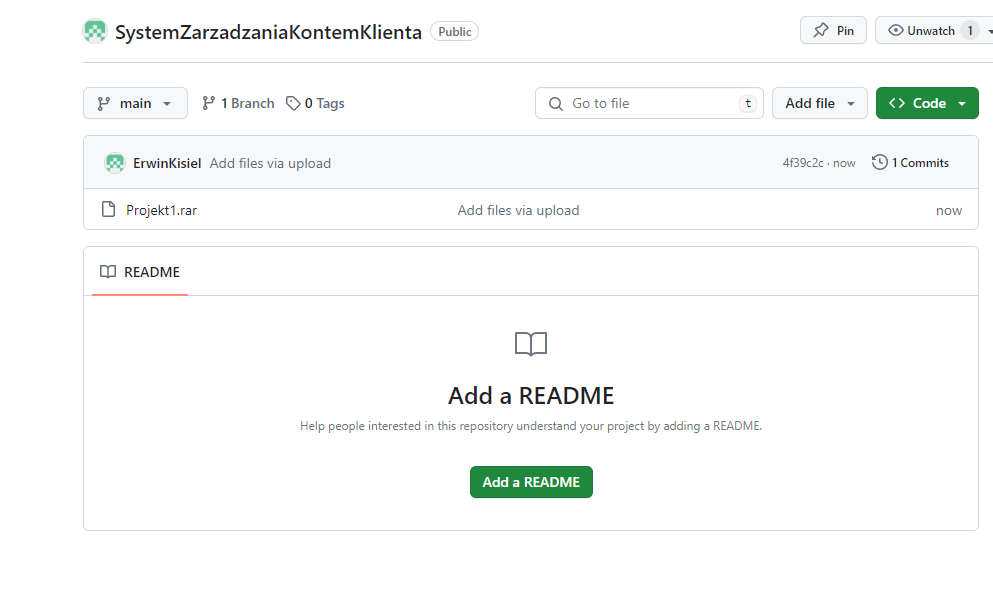
\includegraphics[width=\textwidth]{Repozytorium.png}
      \caption{Repozytorium na GitHub}
    \label{fig:example}
\end{figure}

\newpage
\chapter{Prezentacja warstwy użytkowej}
Projekt systemu zarządzania kontem klienta jest zrealizowany jako aplikacja konsolowa. To znaczy że logika jak i działanie programu jest napisane w języku C\#. Program nie posiada dodatkowego interfejsu graficznego a obsługuje się go za pomocą klawiszy z klawiatury. 
Przedstawiam zrzuty ekranu pokazujące działanie programu.

\section{Ekran powitalny}

\begin{figure}[h]
    \centering
    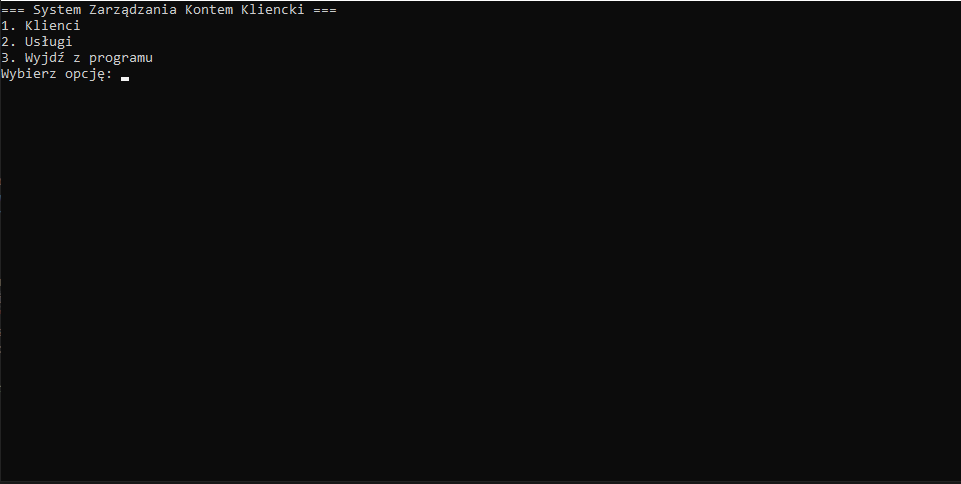
\includegraphics[width=\textwidth]{EkranPow.png}
      \caption{Wybór wyświetlania klienta lub usług}
    \label{fig:example}
\end{figure}

Po uruchomieniu programu w konsoli pokazuje się ekran powitalny z nazwą programu i możliwością przejścia do zakładki klienci lub usługi jest też możliwość zakończenia programu. 

\newpage

\section{Zarządzanie Klientami}

\begin{figure}[h]
    \centering
    \includegraphics[width=\textwidth]{ZarządzanieKlientami.png}
      \caption{Wybór operacji na koncie klienta}
    \label{fig:example}
\end{figure}

Po przejściu do zakładki klientckiej pokazuje się ekran powitalny z menu wyboru odpowiedniej operacji. 

\subsection{Wyświetlanie informacji o klientach}
\begin{figure}[h]
    \centering
    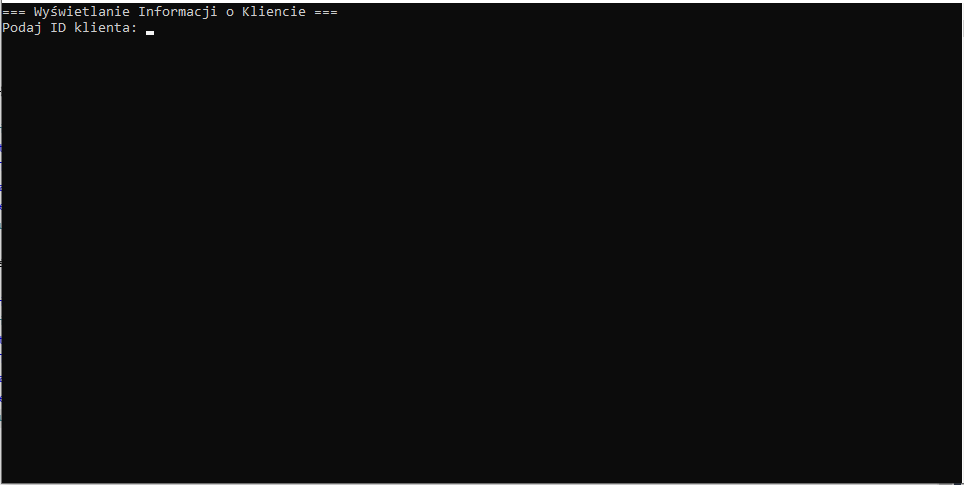
\includegraphics[width=\textwidth]{WysInf.png}
      \caption{Wprowadzanie ID klienta}
    \label{fig:example}
\end{figure}

Wybierając opcję wyświetlenia informacji o kliencie program poprosi o podanie ID klienta którego chcemy wyświetlić.

\subsubsection{Wybór odpowiedniego klienta}
\begin{figure}[h]
    \centering
    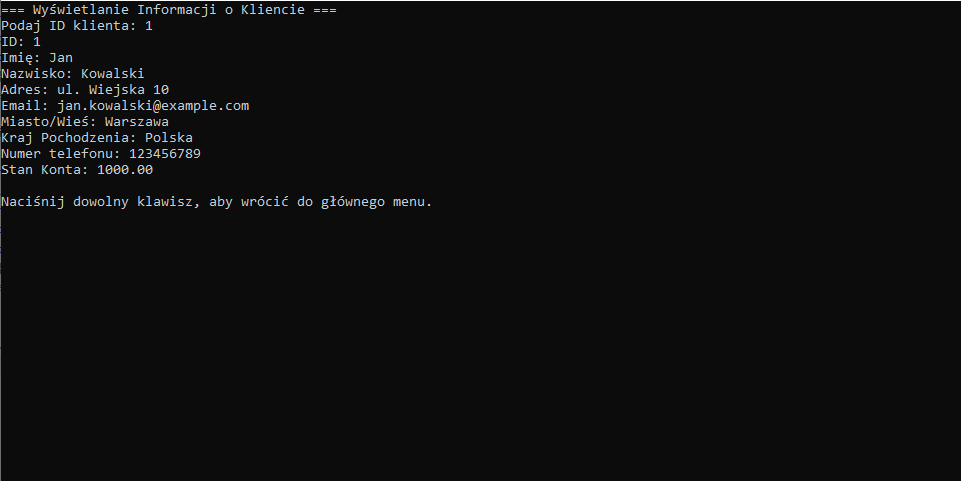
\includegraphics[width=\textwidth]{WysInf1.png}
      \caption{Przedstawienie danych klienta}
    \label{fig:example}
\end{figure}

Po wybraniu odpowiedniego klienta zostaną wyświetlone wszystkie dane pobrane z bazy danych. 

\subsubsection{Wybór klienta którego nie ma w systemie}
\begin{figure}[h]
    \centering
    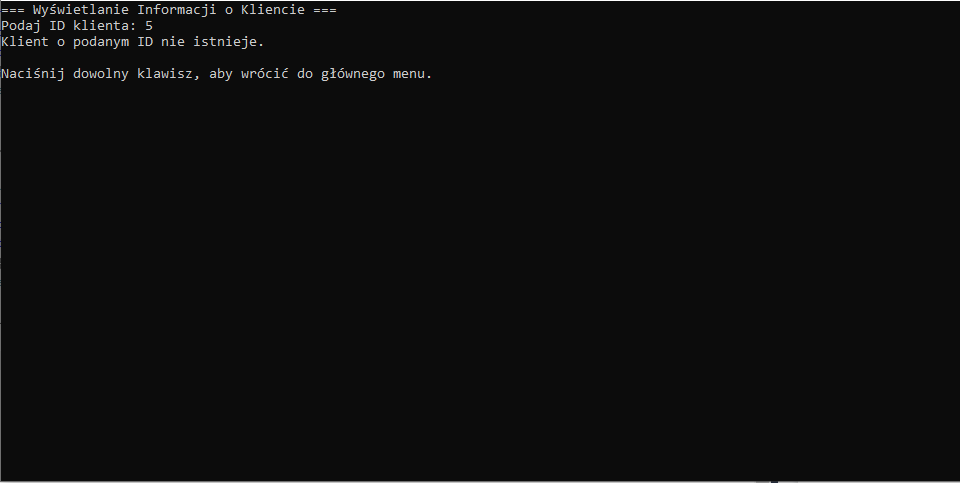
\includegraphics[width=\textwidth]{WysInfBrak.png}
      \caption{Brak klienta o wybranym ID}
    \label{fig:example}
\end{figure}

Jeśli zostanie wybrany klient którego nie ma w systemie program zwróci odpowiednią informację i będziemy mieć możliwość wyszukać ponownie klienta. 

\newpage

\subsection{Dodawanie klienta}


\begin{figure}[h]
    \centering
    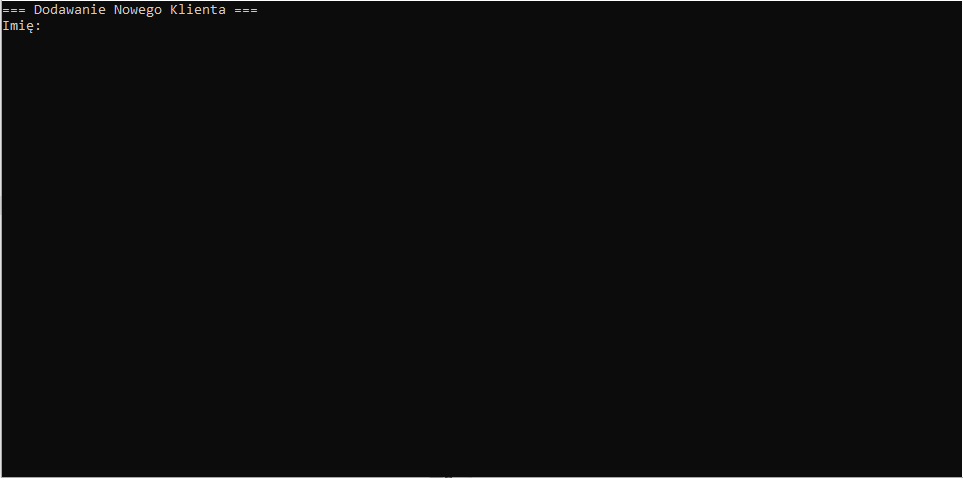
\includegraphics[width=\textwidth]{DodawanieKlienta.png}
      \caption{Możliwość dodania nowego klienta}
    \label{fig:example}
\end{figure}

Wybierając opcje dodania klienta system poprosi nas o wpisanie wszystkich wartości potrzebnych żeby dodać klienta do systemu. 

\subsubsection{Dodanie klienta dane wprowadzone poprawnie}
\begin{figure}[h]
    \centering
    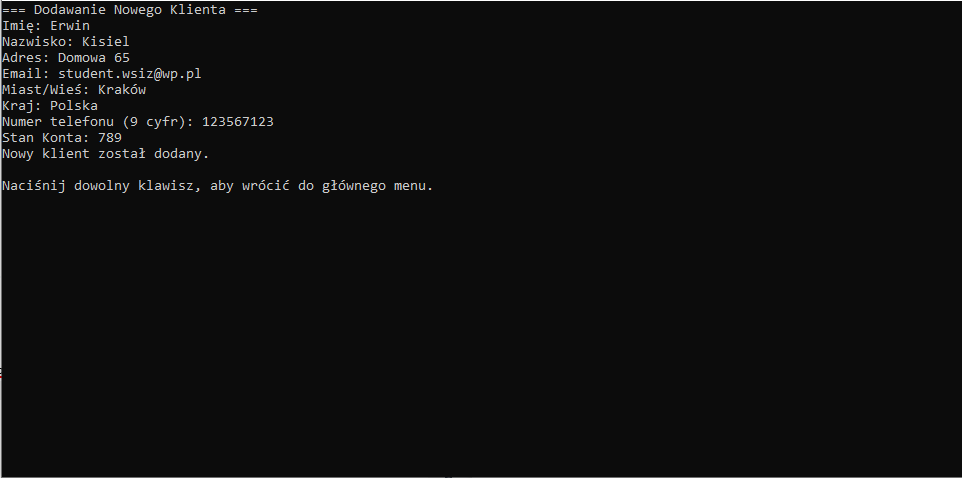
\includegraphics[width=\textwidth]{DodawanieKlientaPop.png}
      \caption{Dodanie klienta do systemu}
    \label{fig:example}
\end{figure}

Po wpisaniu poprawnych danych klient zostanie dodany do systemu automatycznie zostanie mu nadany kolejny numer id.
\newpage
\subsubsection{Dodanie klienta dane wprowadzone błędnie}
\begin{figure}[h]
    \centering
    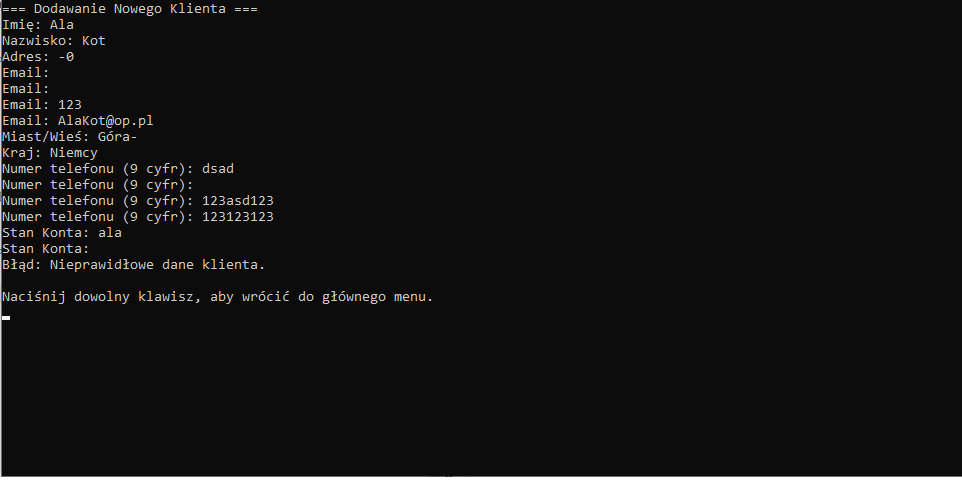
\includegraphics[width=\textwidth]{DodawanieKlientaBle.png}
      \caption{Błąd dodania klienta do systemu}
    \label{fig:example}
\end{figure}

Dodając klienta możemy pomylić się w wielu miejscach dlatego program pozwoli nam przejść dalej lub ponowi możliwość wpisania danej wartości jeśli w miejsce wymagane zostanie wpisana pusta wartość program przejdzie dalej niestety dodawanie zakończy sie niepowodzeniem i trzeba będzie powtórzyć jednak jeśli ktoś się pomyli podczas wpisywania numeru telefonu wpisze więcej cyfr lub doda niedozwolony znak program poprosi go o ponowne wpisanie danej wartości. 

\subsection{Aktualizowanie danych klienta}

\begin{figure}[h]
    \centering
    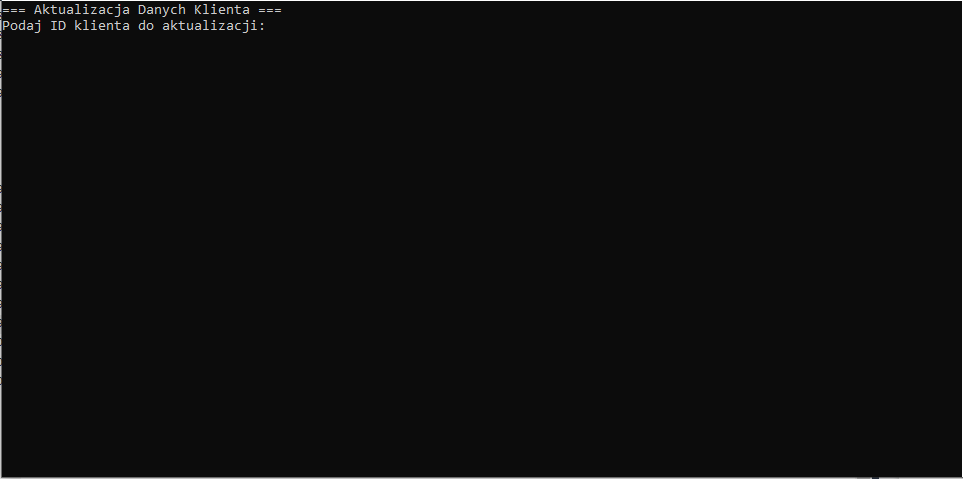
\includegraphics[width=\textwidth]{AktualizacjaDanych.png}
      \caption{Możliwość aktualizacji błędnych danych}
    \label{fig:example}
\end{figure}

Wybierając opcję aktualizacji danych kliencie program poprosi o podanie ID klienta którego chcemy wyświetlić.

\subsubsection{Aktualizowanie danych klienta dane wprowadzone poprawnie}

\begin{figure}[h]
    \centering
    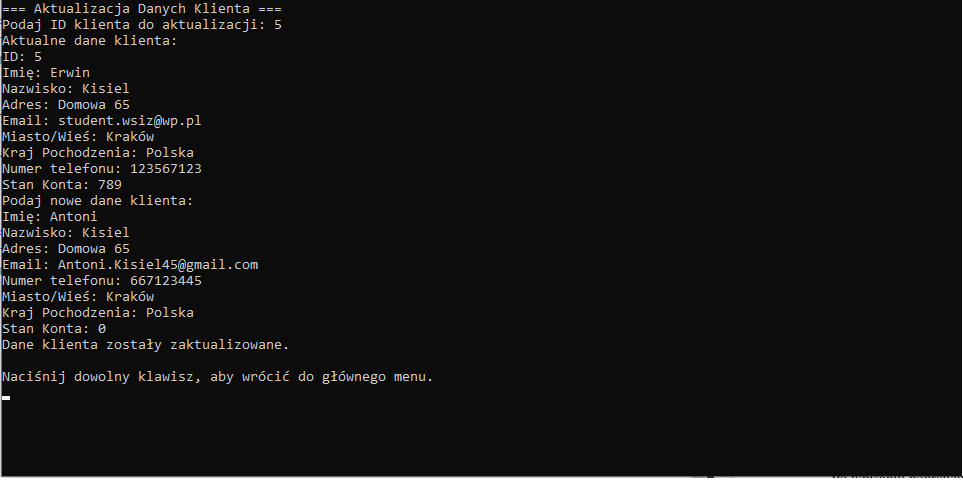
\includegraphics[width=\textwidth]{AktualizacjaDanychPop.png}
      \caption{Możliwość aktualizacji błędnych danych}
    \label{fig:example}
\end{figure}

Po wybraniu klienta którego dane chcemy zaktualizować dostajemy podgląd na dane jakie aktualnie posiada klient i na ich podstawie może wpisać poprawione informacje. 

\subsubsection{Aktualizowanie danych klienta dane wprowadzone błędnie}

\begin{figure}[h]
    \centering
    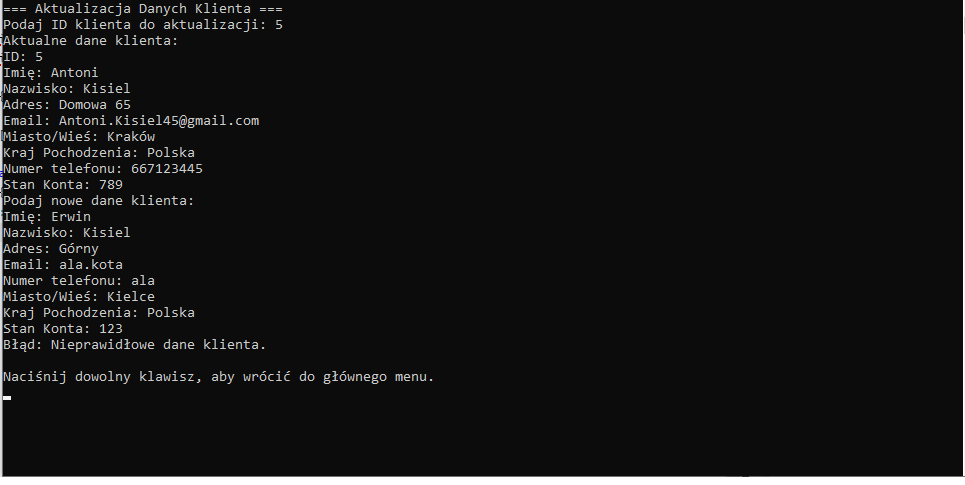
\includegraphics[width=\textwidth]{AktualizacjaDanychNeg.png}
      \caption{Możliwość aktualizacji błędnych danych}
    \label{fig:example}
\end{figure}

Program wykrywa dane które się nie zgadzają nie przedstawia błędu nie prosi też o wpisanie ponownie danej wartości dopiero pod koniec przekazuje że dane nie zostały zaktualizowane i pokazuje błąd. Użytkownik musi od nowa aktualizować dane tym razem bez błędu. 

\subsubsection{Weryfikacja zaktualizowanych danych}

\begin{figure}[h]
    \centering
    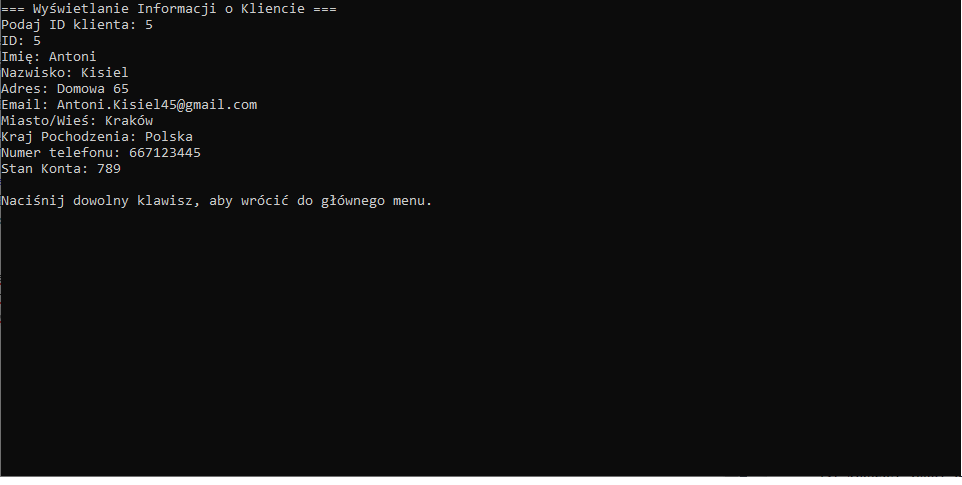
\includegraphics[width=\textwidth]{AktualizacjaDanychWer.png}
      \caption{Weryfikacja danych klienta}
    \label{fig:example}
\end{figure}

Dane klienta zostały zaktualizowane podczas poprawnego wprowadzenia wartości do systemu za to drugim razem po wykonaniu błędu system już nie zmienił wartości. 

\subsection{Usuwanie danych klienta}

\begin{figure}[h]
    \centering
    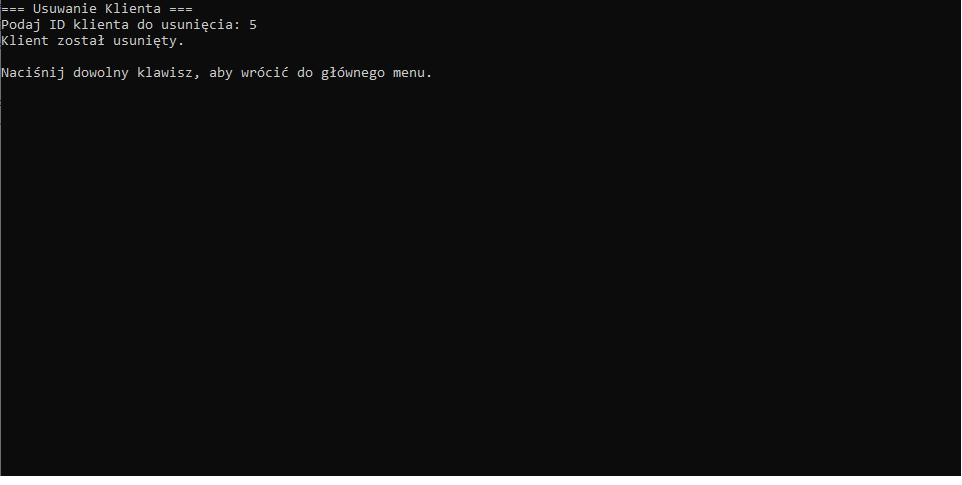
\includegraphics[width=\textwidth]{UsuwanieKlienta.png}
      \caption{Możliwość usuwania klienta z systemu}
    \label{fig:example}
\end{figure}

Wybierając opcję usuwania informacji o kliencie program poprosi o podanie ID klienta którego chcemy usunąć.

\subsubsection{Weryfikacja usuniętych danych klienta}
\begin{figure}[h]
    \centering
    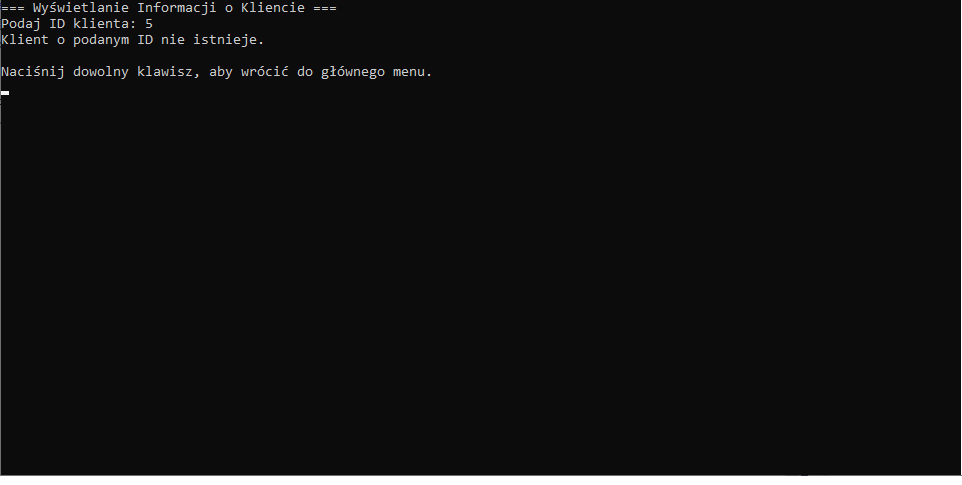
\includegraphics[width=\textwidth]{PotwierdzenieUsu.png}
      \caption{Potwierdzenie usunięcia}
    \label{fig:example}
\end{figure}

\section{Zarządzanie Usługami}

\begin{figure}[h]
    \centering
    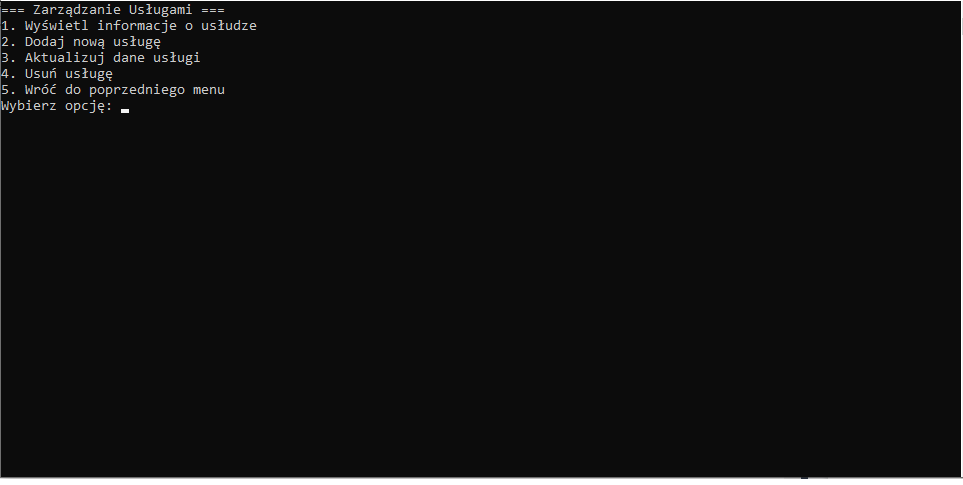
\includegraphics[width=\textwidth]{ZarzadUslug.png}
      \caption{Prezentacja opcji w usługach}
    \label{fig:example}
\end{figure}
Po przejściu do zakładki z usługami pokazuje się ekran powitalny z menu wyboru odpowiedniej operacji. 

\subsection{Wyświetlanie informacji o usługach}

\begin{figure}[h]
    \centering
    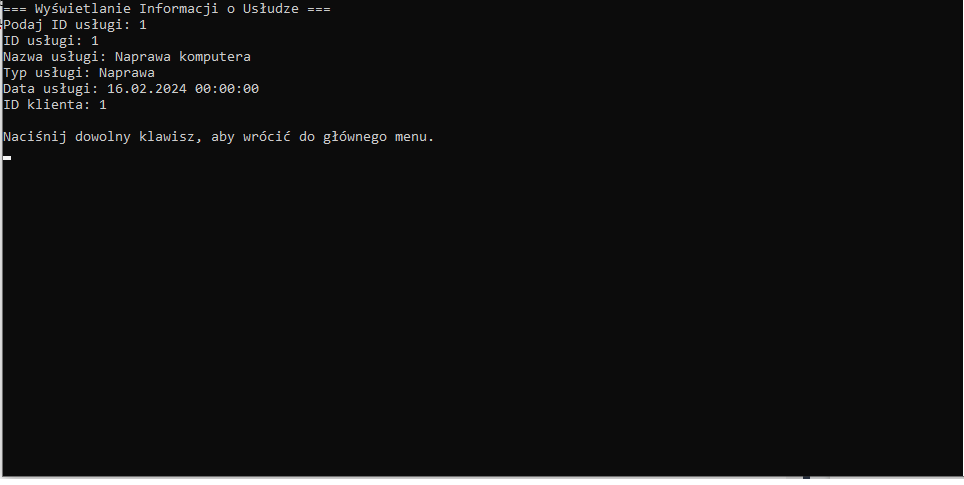
\includegraphics[width=\textwidth]{WysInfUslug.png}
      \caption{Przedstawienie danych usługi}
    \label{fig:example}
\end{figure}

Wybierając opcję wyświetlenia informacji o usługacg program poprosi o podanie ID klienta którego chcemy wyświetlić.

\subsection{Dodawanie usług}
\begin{figure}[h]
    \centering
    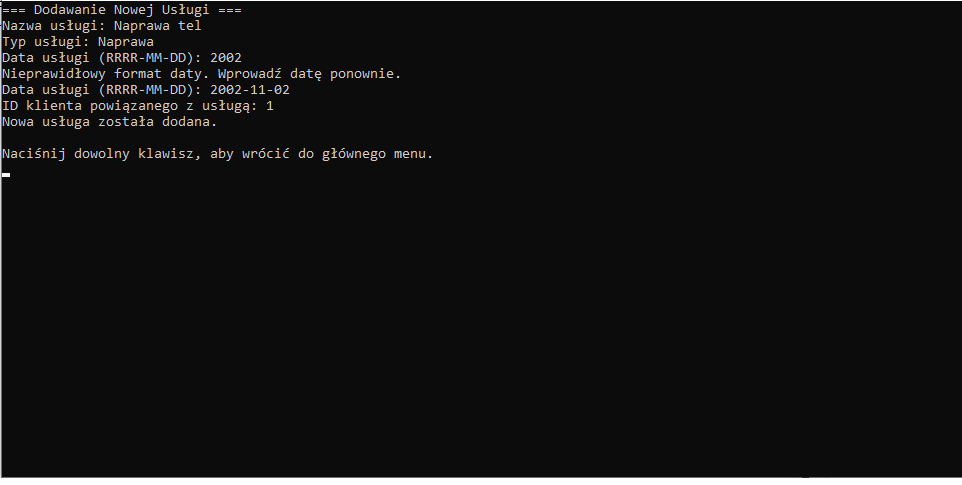
\includegraphics[width=\textwidth]{DodawanieUslug.png}
      \caption{Dodanie usługi do systemu}
    \label{fig:example}
\end{figure}

\newpage
Wybierając opcje dodania usługi system poprosi nas o wpisanie wszystkich potrzebnych danych.

\subsection{Aktualizacja danych w usługach}
\begin{figure}[h]
    \centering
    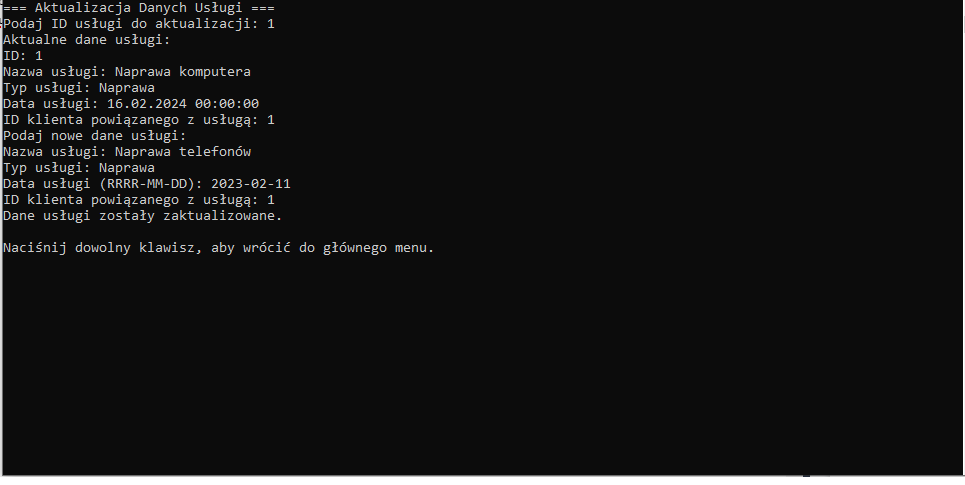
\includegraphics[width=\textwidth]{AktualizacjaDanychUslug.png}
      \caption{Zaktualizowanie danych o usłudze}
    \label{fig:example}
\end{figure}

Po wybraniu usługi którą chcemy zaktualizować dostajemy podgląd i na jego podstawie może wpisać poprawione informacje. 



\subsection{Usuwanie usług}
\begin{figure}[h]
    \centering
    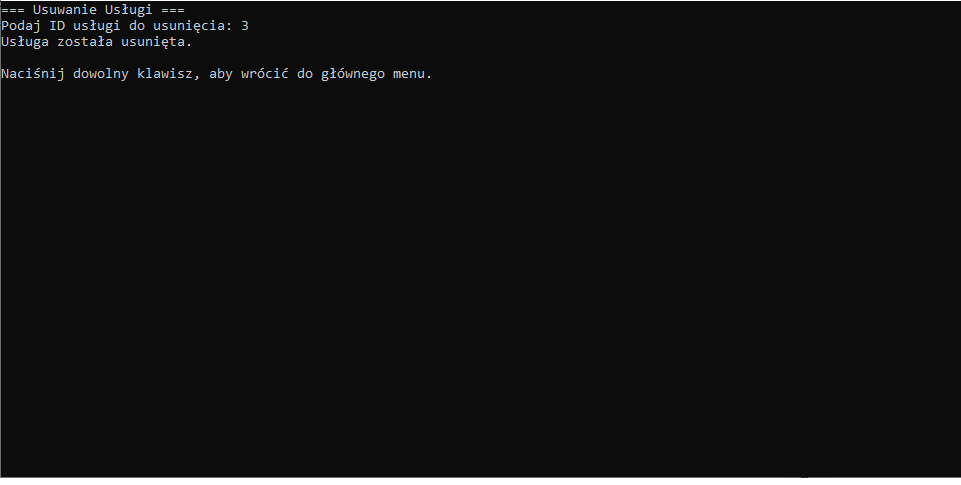
\includegraphics[width=\textwidth]{UsuwanieUslug.png}
      \caption{Usunięcie usługi}
    \label{fig:example}
\end{figure}

Wybierając opcję usuwania informacji o usłudze program poprosi o podanie ID dzięki niemu może odnaleźć usługę do usunięcia.
\newpage
\chapter{Podsumowanie}

\section{Plany rozbudowy aplikacji}

W dalszych planach rozbudowy systemu zarządzana kontem klienta zostanie wprowadzone wiele nowych funkcji oraz usprawnień mających na celu zwiększyć użyteczność, efektywność, bezpieczeństwo oraz przejrzystość.
System oparty jest na aplikacji konsolowej w planach jest wprowadzenie interfejsu graficznego (GUI) co znacząco poprawy jakość korzystania z tego systemu. Zostanie dodany panale administracyjny dla pracowników obsługi klienta, panel zarzadzania użytkownikami. Zwiększymy bezpieczeństwo systemu przez dodanie dodatkowych zabezpieczń oraz systemu autoryzacji. Zostaną także zaimplementowane dodatkowe funkcje raportowania i analizy danych które pozwolą bardziej szczegółowo monitorować aktywność klientów oraz jakość/wydajność usług. 

\section{Podsumowanie zrealizowanych prac}

Realizując projekt "System zarządzania kontem klienta w firmie telekomunikacyjnej" w języku C\# głównym celem zostało stworzenie systemu przyjaznego konsultantowi który potrzebuje pozyskać konkrente informacje na temat klienta. Dzięki funkcjonalności aplikacja pozwala sprawdzać informacje o klientach i usługach dodawać, usuwać a nawet modyfikować dane. Zostało stworzone proste środowisko do wykonywania potrzebnych operacji. Praca nad systemem została zakończona sukcesem. 
\newpage

% *************** Bibliografia ***************
\begin{thebibliography}{6}
\addcontentsline{toc}{chapter}{Bibliografia}
%dodanie wpisu do spisu bibliograficznego

\bibitem{www-1} https://pl.wikipedia.org/wiki/C\_Sharp z dnia 4.02.2024
\bibitem{www-2} https://learn.microsoft.com/pl-pl/dotnet/csharp/ z dnia 15.02.2024

\bibitem{etykieta1}Jesse Liberty, Ian Griffiths, Matthew E. Adams, {\it C\#. Programowanie}, Helion,  2005.
\bibitem{etykieta2}Andrew Stellman, Jennifer Greene, {\it Head First C\# (Head First)}, Helion,  2009.
\end{thebibliography}
\newpage

% *************** Zakończenie ***************
% *************** Zakończenie ***************

%***************************************************************************************
% W tym miejscu znajdują się polecenia odpowiedzialne za tworzenie
% spisu ilustracji, spisu treści oraz streszczenia pracy
%***************************************************************************************

%spis rysunków
\addcontentsline{toc}{chapter}{Spis rysunków}
\listoffigures
\newpage


% *************** Koniec pliku back.tex ***************


\end{document}
% *************** Koniec pliku szablon.tex ***************
